%part 4
%	\chapter{Изучение особенностей магнитооптической структуры синхротронов NICA и Nuclotron с учетом %ускорения поляризованных пучков и модернизация магнитооптической структуры Nuclotron с учётом возможности %изучения ЭДМ}\label{ch:EDM}

%	\chapter{Изучение особенностей магнитооптической структуры синхротронов для ускорения поляризованных пучков с учётом возможности изучения ЭДМ}\label{ch:EDM}
	\chapter{Возможности изучения ЭДМ легких поляризованных пучков заряженных частиц}\label{ch:EDM}
 
\par Известная проблема физики состоит в объяснении барионной асимметрии, то есть наблюдаемым преобладанием материи над антиматерией. До сих пор, существующие физические законы не способны полностью объяснить такой дисбаланс. В работе 1967 год А. Д. Сахаровым были сформулированы общие необходимые условия для наличия барионной асимметрии: 1) Нарушение закона сохранения барионного заряда; 2) Нарушение C- и CP-симметрии; 3) Нарушение на ранних этапах формирования Вселенной термодинамического равновесия \cite{sakharov}. Согласно второму условию, "\textit{Возникновение С-асимметрии по нашей гипотезе является следствием нарушения СР-инвариантности при нестационарных процессах расширения горячей Вселенной на сверхплотной стадии, которое проявляется в эффекте различия парциальных вероятностей зарядово-сопряженных реакций}".  Ранее в 1958 году С. Окубо теоретически показал такой эффект при рассмотрении распада сигма гиперона $\Sigma^{+}$ и его античастицы $\bar{\Sigma}^{+}$. Позднее в 1964 году Д. Кронин и В. Фитч экспериментально обнаружили нарушение CP-инвариантности слабого взаимодействия в процессах распада нейтральных каонов $K_{2}^{0}$ на два пиона $\pi^{+}, \pi^{-}$ \cite{CP}, за что в 1980 году были удостоены нобелевской премии по физике. 

\par В современной Стандартной модели частиц P-\cite{P-violation} и CP-симметрии нарушаются. Источником CP-нарушения является наличие комплексной фазы в матрице смешивания кварков Кабиббо-Кабаяси-Маскава для слабых взаимодействий \cite{CKM} и коэффициента $\theta_{\text{QCD}}$ в лагранжиане квантовой хромодинамики \cite{CPstrong}, однако не обнаружено CP-нарушений в сильных взаимодействиях. Согласно CPT-теореме, CP-инвариантность эквивалентна T-инвариантности. Источником такого нарушения может являться ненулевой электрический дипольный момент (ЭДМ) элементарных частиц, фундаментальное свойство материи и обусловленное неоднородностью распределения заряда внутри частицы. Поскольку ЭДМ представляется полярным вектором, а не псевдовектором, то для него нарушается как P-, так и T-инвариантность, что показано на Рис. \ref{fig:4edmpt}.  Величина ЭДМ в Стандартной Модели слишком мала для экспериментального детектирования и находится на уровне $\abs{d_{n}}< 10^{-30}-10^{-32}$ $e\cdot \text{см}$ для нейтрона \cite{EMD_overview}. Возможность его существования была сформулирована в заметке 1950 Перселл и Рэмси \cite{EDM}, однако ненулевое ЭДМ пока точно не обнаружено. Другие теоретические модели, такие как Суперсимметричные (SUSY), также предсказывают наличие ЭДМ, но на уровне $\abs{d_{n}}< 10^{-27}-10^{-29}$ $e\cdot \text{см}$ для нейтрона, которые оставляют существенную надежду на экспериментальное обнаружение. Стоит отметить, что и таких точностей пока достигнуто не было, а сделаны только существенные ограничения для нейтрального нейтрона, впервые появившиеся в работе Н. Рамси и его коллег $\abs{d_{n}}< 5\times10^{-20}$ $e\cdot \text{см}$ ($90\%$ C.L.) \cite{NeutronEDM}, текущее ограничение находится на уровне $\abs{d_{n}}< 1.8\times 10^{-26}$ $e\cdot \text{см}$ ($90\%$ C.L.), что получено в работе nEDM \cite{neutron_EDM_current}.

\begin{figure}
	\centering
	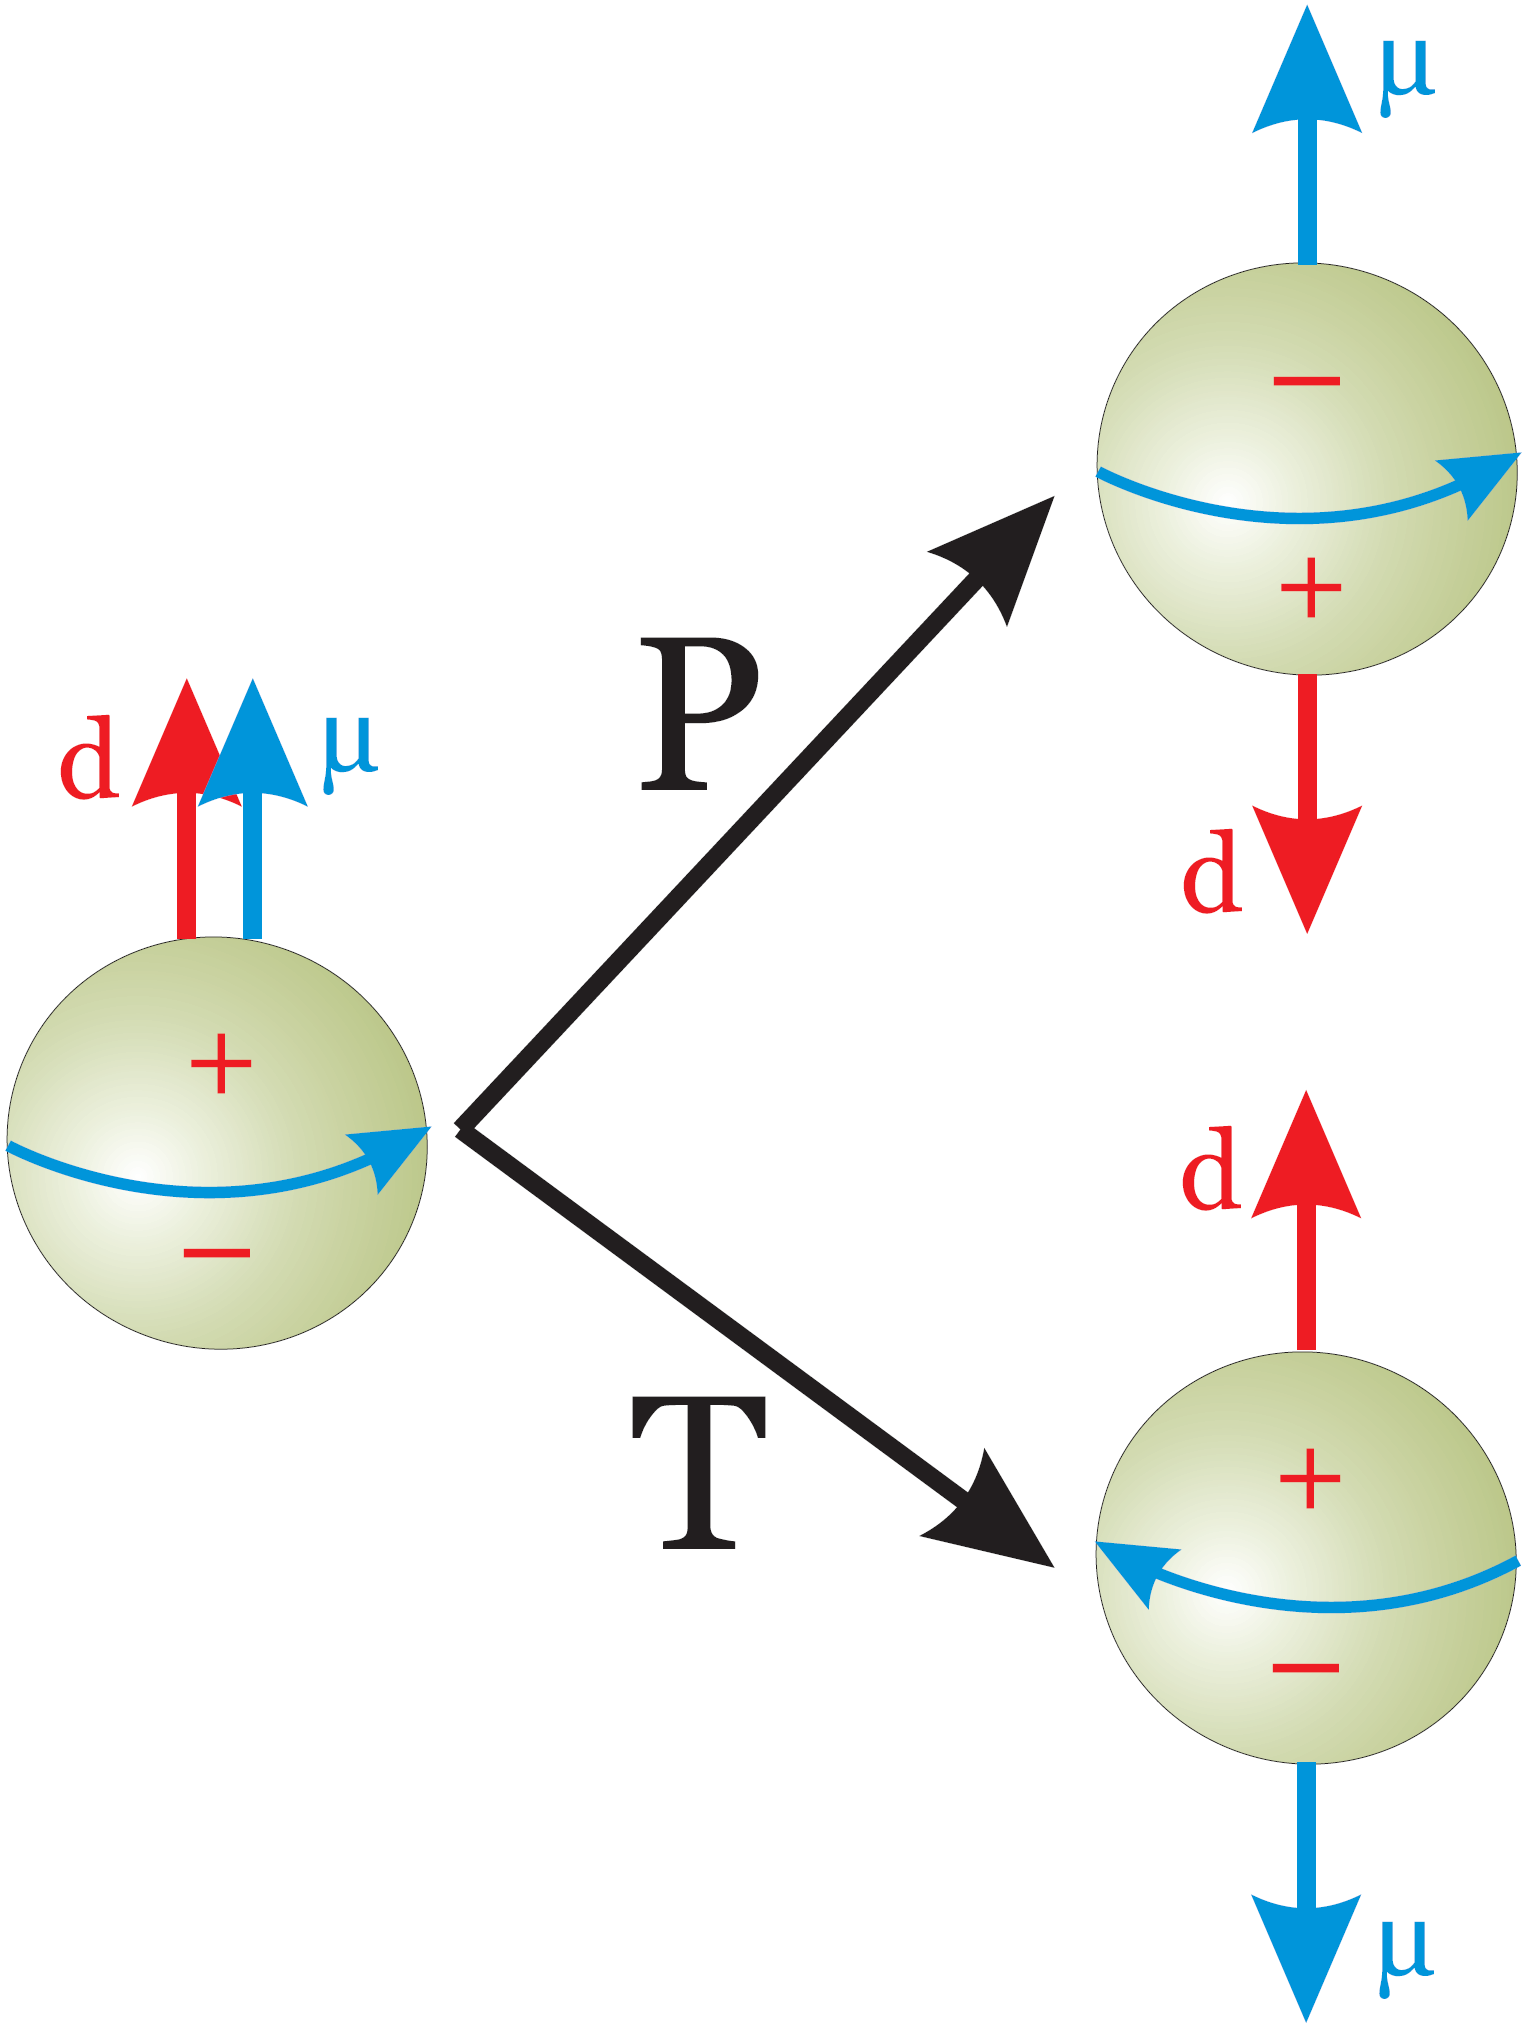
\includegraphics[width=0.4\linewidth]{images/4_EDM_P_T}
	\caption{Схематическое изображение нарушение P- и Т-симметрии ненулевым электрическим дипольным моментом.}
	\label{fig:4edmpt}
\end{figure}

\par Изучение ЭДМ нейтрона, а также нейтральных атомов удобно сохранением их положения при действии внешних магнитных и электрических полей. В случае заряженных частиц происходит движение, согласно силе Лоренца, что и приводит к необходимости применения ускорительных установок, позволяющих длительное накопление пучка с заданными параметрами и выступающих в роли накопительного кольца. Наиболее интересными и перспективными направлениями выглядит изучение ЭДМ протона и дейтрона. 

\par Обнаружение ЭДМ-эффекта может быть осуществлено по изучению поведения спина во внешних электромагнитных поля. Важным является отличие свойства индивидуальной частицы -- спина и пучка -- поляризации. Возможность изучения спина ансамбля частиц определяется теоремой Эренфеста \cite{Ehrenfest} и состоит в том, что уравнения для средних значений квантовых наблюдаемых величин формально тождественны уравнениям классической механики, если все величины заменить на соответствующие средние значения. Применение этой теоремы к чисто квантовой величине -- спин, позволяет оперировать понятием -- поляризации пучка, где усреднение может осуществляться как по количеству частиц, так и по оборотам. Классическое уравнение описывающее эволюцию вектора спина было получено Телегди, Баргманн, Мишель в 1959 году \cite{TBMT}, с учётом одноименной прецессии Томаса. Вращение осуществляется за счёт наличия как магнитного дипольного момента (МДМ), так и ЭДМ 

\begin{equation}	
\begin{aligned} 
	\dv{{\vec{S}}}{t} &=\left(\vec{\Omega}_{\textrm{MDM}}+\vec{\Omega}_{\textrm{EDM}}\right) \times \vec{S}, \\
	\vec{\Omega}_{\textrm{MDM}}&=-\frac{q}{m \gamma}\left\{(\gamma G+1)\vec{B}_{\perp}+(G+1)\vec{B}_{\parallel}-\left(\gamma G+\frac{\gamma}{\gamma+1}\right) \frac{\vec{\beta} \times \vec{E}}{c}\right\}, \\
	\vec{\Omega}_{\textrm{EDM}}&=-\frac{q \eta}{2 m}\left(\vec{\beta} \times \vec{B}+\frac{\vec{E}}{c}-\frac{\gamma}{\gamma+1}\frac{\vec{\beta}}{c}\left(\vec{\beta}\cdot\vec{E}\right)\right), \quad G=\frac{g-2}{2},
\end{aligned}
\label{eq:T-BMT}
\end{equation}	

\noindent где $\vec{\Omega}_{\textrm{MDM}}, \vec{\Omega}_{\textrm{EDM}}$ -- угловые частоты обусловленные наличием МДМ и ЭДМ; $q, m, G$ -- заряд, масса и магнитная аномалия; $\beta$ -- нормализованная скорость; $\gamma$ -- Лоренц-фактор; $d =~\eta \frac{q}{2mc}s$ -- ЭДМ фактор, $s$ -- спин. Уравнение содержит 2 слагаемых, одно обусловлено наличием МДМ, другое – ЭДМ соответственно \cite{silenko:edm}. Главным образом, ЭДМ пропорционален силе Лоренца, которая отлична от нуля в элементах с ненулевой кривизной и равняется нулю на прямых участках. 

\par Для непосредственного измерения ЭДМ-компоненты, влияние МДМ на спин должно быть нивелировано. Это может быть достигнуто, во-первых, полным занулением МДМ-члена в каждой точке кольца, такой метод получил название \textit{замороженный спин} (\textit{frozen spin}). Либо интегрально, когда элементы одного типа последовательно компенсируются другого, такой подход получил название \textit{квази-замороженный спин} (\textit{quasi-frozen spin}) \cite{QFS}.

\par На сегодняшний день исследование поляризованных пучков заряженных частиц велось в нескольких ускорительных центрах \cite{EDM_Yellow}. Первоначально, с мюонами на эксперименте $g-2$ в Брукхейвенской Национальной Лаборатории в США (BNL, USA) \cite{g-2}. Позднее, в 2004 году изложена идея измерения дейтрона с использованием метода замороженного спина коллаборацией srEDM, также в БНЛ \cite{Farley:edm}. Предлагалось измерение увеличения абсолютного значения вертикальной компоненты поляризации. В 2008 году, исследования проводились в накопительном кольце COSY (COoler SYnchrotron) в Исследовательском центре “Юлих” (Forschungszentrum Jülich GmbH, Германия) \cite{Farley:edm}.

\par Новым крупным центром станет комплекс ОИЯИ NICA-Nuclotron в городе Дубна, Россия, с возможностью всестороннего изучения спиновой физики. В том числе уже упомянутое изучение ЭДМ заряженных частиц, коллайдерные эксперименты с симметричными и асимметричными пучками с целью изучения проблемы "спинового кризиса"\cite{ST_Filatov}, а также поиск аксиона \cite{Axion_Nikolaev}. В данной главе будут рассмотрены способы создания квази-замороженного спина в периодических структурах и возможность их реализации. Кроме того, будет измерен не абсолютный рост вертикальной компоненты, а частота, что получило название метод частотной области (frequancy domain method) \cite{FDM}.

\par Помимо, рассмотренного в Главах \ref{ch:dual}-\ref{ch:resonant}, коллайдера NICA, в ускорительный комплекс также входит установка Nuclotron \cite{nuclotron24}. Данный синхротрон предназначен как для самостоятельных экспериментов на выведенной мишени BM@N и изучения управления поляризацией, так и для использования в качестве инжектора поляризованного пучка протонов и дейтронов в коллайдер NICA. Однако, установка была введена в эксплуатацию в 90-е годы \cite{baldin:nuclotron} и может быть модернизирована с использованием новых современных магнитооптических элементов, производимых непосредственно в ОИЯИ г. Дубна \cite{korovkin:nica_magnets}. Для расширения возможностей Nuclotron в качестве самостоятельной машины рассматривается возможность изучения ЭДМ легких заряженных частиц. Такие прецизионные эксперименты возможны на ускорителе, работающем в режиме накопительного кольца с целью долгого удержания сгустка на орбите и накоплению достаточной статистики эксперимента. 

\par Возможность исследования ЭДМ с применением метода квази-замороженного спина возможна также и на установке, изначально для этого не предназначенной. Однако, поскольку для компенсации влияния МДМ необходимо использование элементов с электрическим полем, требуется дополнительное место для их расположение. Такое может быть достигнуто путем введения обводных каналов. Это возможно в том числе в кольце коллайдера NICA.

\par В экспериментах по измерению ЭДМ ключевым является обеспечение высокого показателя времени когерентности (SCT — Spin Coherence Time) порядка 1000 секунд, что было получено в кольце COSY \cite{AGSproposal}. В течение такого времени когерентный поляризованный пучок удерживается на орбите. Таким образом, для моделирования структуры с возможностью исследования ЭДМ необходимо гарантировать стабильность спиновой динамики вдоль всего кольца, что является отдельной задачей, наравне с обеспечением орбитальной стабильности пучка.

\section{Орбитальная и спиновая динамика в электромагнитных полях}\label{sec:EDM/requirements/deflector}

\par Рассмотрим как орбитальное, так и спиновое движение в электромагнитных полях в обобщенном виде. Для орбитального вращения в поперечном магнитном поле согласно уравнению Лоренца

\begin{equation} 
qc\vec{\beta}\times{\vec{B}}_\bot={\vec{\Omega}}_p^{\textrm{B}}\times\vec{p},
\label{eq:lorenz}
\end{equation}

\noindent где $q$ -- заряд, $c$ -- скорость света, $\vec{\beta}$ -- вектор относительной скорости, ${\vec{B}}_\bot$ -- поперечное магнитное поле, $\vec{p}$ -- импульс частицы, ${\vec{\Omega}}_p^{\textrm{B}}$ -- вектор угловой скорости (индексы означают, что происходит вращение импульса в магнитном поле). Учтем, что импульс частицы представим в виде $\vec{p}\ =\ \gamma mc\vec{\beta}$, тогда ур.\ref{eq:lorenz}а с учетом перестановки векторного произведения получаем

\begin{equation}	
qc\vec{\beta}\times{\vec{B}}_\bot=-mc\gamma\vec{\beta}\times{\vec{\Omega}}_p^{\textrm{B}},
\end{equation}

\noindent для угловой скорости

\begin{equation} \label{eq:omega_pB}
 {\vec{\Omega}}_p^{\textrm{B}}=-\frac{q}{m\gamma}{\vec{B}}_\bot.
\end{equation} 

\begin{figure}[!h]
  \centering
	\includegraphics*[width=0.49\columnwidth]{4_orbital_B}
	\includegraphics*[width=0.49\columnwidth]{4_orbital_E}
   \caption{Вращение положительно заряженной частицы а) в магнитном поле; б) электростатическом поле.}
   \label{fig:4_orbital_B_E}
\end{figure}

\par Для заряженной частицы в электростатическом дефлекторе, выполняющего функцию поворота всегда соблюдается условие $\vec{p} \bot \vec{E}$, тогда происходит движение по окружности (рис.\ref{fig:4_orbital_B_E}б) и аналогично ур.\ref{eq:lorenz}

\begin{equation}
q{\vec{E}}_\bot={\vec{\Omega}}_p^{\textrm{E}}\times\vec{p},
\end{equation} 

\noindent где ${\vec{E}}_\bot$ – электростатическое поле перпендикулярное импульсу, ${\vec{\Omega}}_p^{\textrm{E}}$ – вектор угловой скорости (индексы означают, что происходит вращение импульса в электростатическом поле)

\begin{equation}
q{\vec{E}}_\bot=mc\gamma{\vec{\Omega}}_p^{\textrm{E}}\times\vec{\beta}.
\end{equation} 

\noindent Для угловой скорости с учётом векторного произведения $\vec{v}=\vec{\omega}\times\vec{r}, \vec{\omega}=\frac{\vec{r}\times\vec{v}}{(\vec{r},\vec{r})}$

\begin{equation}
{\vec{\Omega}}_p^{\textrm{E}}=\frac{q}{mc}\frac{\vec{\beta}\times{\vec{E}}_\bot}{\gamma(\vec{\beta},\vec{\beta})}=\frac{q}{m\gamma}\frac{\vec{\beta}\times{\vec{E}}_\bot}{c\beta^2}\ \ \ 
\label{eq:orbital_E}
\end{equation}

\par Рассмотрим теперь вращение спинового вектора под действием МДМ, описываемого уравнением Т-БМТ \ref{eq:T-BMT} относительно вектора импульса

\begin{equation}
{\vec{\omega}}_p^{\textrm{B}}={\vec{\Omega}}_{\textrm{MDM}}^\textrm{B}-{\vec{\Omega}}_p^{\textrm{B}}=-\frac{q}{m\gamma}\left(\gamma G+1\right){\vec{B}}_\bot+\frac{q}{m\gamma}{\vec{B}}_\bot=-\frac{q}{m}{G\vec{B}}_\bot.
\end{equation}

\noindent Величина $\nu_s^{\textrm{B}}$ -- \textit{спин-тюн} (\textit{spin-tune}) является скалярной величиной и отражает во сколько раз поворот вектора спина больше поворота вектора импульса

\begin{equation} 
\nu_s^{\textrm{B}}=\frac{\left|{\vec{\Omega}}_{\textrm{MDM}}^{\textrm{B}}-{\vec{\Omega}}_p^{\textrm{B}}\right|}{\left|{\vec{\Omega}}_p^{\textrm{B}}\right|}=\frac{-\frac{q}{m}{G\left|\vec{B}\right|}_\bot}{-\frac{q}{m\gamma}\left|{\vec{B}}_\bot\right|}=\gamma G.
\label{eq:spintune_B}
\end{equation}

\noindent Аналогично для вращения в электростатическом поле
\begin{equation}
\begin{aligned}
{\vec{\omega}}_p^{\textrm{E}}={\vec{\Omega}}_{\textrm{MDM}}^{\textrm{E}}-{\vec{\Omega}}_p^{\textrm{E}}&=\frac{q}{m}\left(G+\frac{1}{\gamma+1}\right)\frac{\vec{\beta}\times\vec{E}}{c}-\frac{q}{mc}\frac{\vec{\beta}\times\vec{E}}{\gamma\beta^2} =\\
&=\frac{q}{mc}\left(G-\frac{1}{\gamma^2-1}\right)\vec{\beta}\times\vec{E}.
\end{aligned}
\end{equation}

\noindent Спин-тюн в электростатическом поле

\begin{equation} 
\nu_s^{\textrm{E}}=\frac{\left|{\vec{\Omega}}_{\textrm{MDM}}^{\textrm{E}}-{\vec{\Omega}}_p^{\textrm{E}}\right|}{\left|{\vec{\Omega}}_p^{\textrm{E}}\right|}=\frac{\frac{q}{mc}\left(G-\frac{1}{\gamma^2-1}\right)\left|\vec{\beta}\times\vec{E}\right|}{\frac{q}{mc}\frac{\left|\vec{\beta}\times\vec{E}\right|}{\gamma\beta^2}}=\gamma\beta^2\left(G-\frac{1}{\gamma^2-1}\right).
\label{eq:spintune_E}
\end{equation}
Примечательно, что спин-тюн как в магнитном поле ур. \ref{eq:spintune_B}, так и  электростатическом ур. \ref{eq:spintune_E} не зависит от величины поля в дефлекторе, а определяется энергией и аномальным магнитным моментом.

\section{Общий концепт квази-замороженной структуры}\label{sec:EDM/requirements/deflector}

\par Сформулируем концепцию квази-замороженной структуры в общем смысле. Перейдем от рассмотрения общего случая вращения спина в магнитном и электрическом поле к непосредственным элементам и поворотным аркам. Первым условием является сохранение конфигурацию замкнутой орбиты, при этом орбитальная траектория остается неизменной от оборота к обороту. Для периодической структуры это условие может быть сформулировано как 

\begin{equation}
	\Phi_p^{\textrm{arc}}+\Phi_{p}^{\textrm{comp}}=\frac{2\pi}{N}\ \ \
	\label{eq:QFS_orbital}
\end{equation}

\noindent где индекс $p$ -- указывает на импульс, $\Phi_p^{\textrm{arc}}$ и $\Phi_{p}^{\textrm{comp}}$ -- суммарное вращение импульса в поворотной арке и компенсаторе спинового вращения, $N$ - периодичность структуры. Для создания накопительного кольца, подходящего как для изучения ЭДМ, так и исследований на более высокой энергии, важно использовать чисто магнитную арку с поперечным ведущим полем, учитывая ограничения максимальной достижимой напряженности электростатического поля. В этом случае используется отдельный соответствующий спиновый компенсатор, который не возмущает орбиту. Окончательно, данные утверждения могут быть сформулированы как $\Phi_p^{\textrm{arc}} = \frac{2\pi}{N}$ и тогда $\Phi_{p}^{\textrm{comp}} = 0$. Для того, чтобы эффективная сила Лоренца равнялась нулю в спиновом компенсаторе, должно быть использовано как электрическое, так и магнитное поле. Из уравнения \ref{eq:QFS_orbital} для углов вращения справедливо

\begin{equation}
	\Phi_{p\textrm{B}}^{\textrm{comp}}+{\Phi}_{p\textrm{E}}^{\textrm{comp}} = 0,\ \ \,
	\label{eq:spin_comp}
\end{equation}

\noindent где $\Phi_{p\textrm{B}}^{\textrm{comp}}$ и ${\Phi}_{p\textrm{E}}^{\textrm{comp}}$ -- суммарное вращение в магнитном и электрическом полях спинового компенсатора. Из уравнения \ref{eq:T-BMT} видно, что максимальная эффективность электростатического поля достигается при радиальном направлении по отношению к вектору импульса. Кроме того, такое поле также эффективно для орбитального вращения, что следует из ур. \ref{eq:orbital_E}.

Второе условие для реализации квази-замороженной структуры -- компенсация МДМ-вращения на одном периоде кольца

\begin{equation}
	\Phi_s^{\textrm{arc}}+\Phi_{s}^{\textrm{comp}}=0,
	\label{eq:QFS_spin}
\end{equation}

\noindent где $\Phi_s^{\textrm{arc}}$ and $\Phi_{s}^{\textrm{comp}}$ -- суммарное вращение спина в поворотной арке и спиновом компенсаторе. Компенсация осуществляется благодаря фундаментальному различию вращения в магнитном и электрическом поле. Используя соотношения из ур. \ref{eq:spintune_B}, \ref{eq:spintune_E}, получаем уравнения связи для углов в чисто магнитном поле поворотной арки  $\Phi_{s}^{\text{arc}} = \nu_{\mathrm{B}_{\perp}}\Phi_{p}^{\text{arc}}$ и магнитном $\Phi_{s\mathrm{B}}^{\text{comp}} = \nu_{\mathrm{B}_{\perp}}\Phi_{p\mathrm{B}}^{\text{comp}}$ и электрическом $\Phi_{s\mathrm{E}}^{\text{comp}} = \nu_{\mathrm{E}}\Phi_{p\mathrm{E}}^{\text{comp}}$ в спиновом компенсаторе. Тогда, для ур. \ref{eq:QFS_spin}

 \begin{equation}
	\begin{aligned}
		\nu_{\mathrm{B}_{\perp}}\Phi_{p}^{\text{arc}} +
		\left(\nu_{\mathrm{B}_{\perp}}\Phi_{p\mathrm{B}}^{\text{comp}} +
		\nu_{\mathrm{E}}\Phi_{p\mathrm{E}}^{\text{comp}} \right) & = \\
		= \nu_{\mathrm{B}_{\perp}} \left( 
		\Phi_{p}^{\text{arc}} +
		\Phi_{p\mathrm{B}}^{\text{comp}} \right) +
		\nu_{\mathrm{E}}\Phi_{p\mathrm{E}}^{\text{comp}}  & = 0.
		\label{eq:deflection}
	\end{aligned}
\end{equation}

\par Окончательно, согласно первому и второму условию квази-замороженного спина, для угла вращения в магнитном или электрическом поле в компенсаторе МДМ-вращения

\begin{equation}
	\Phi_{p\mathrm{E}}^{\textrm{comp}} = - \Phi_{p\mathrm{B}}^{\textrm{comp}} = {\Phi}_{p}^{\text{arc}}\frac{\gamma^2 G}{G+1} =\frac{2\pi}{N}\frac{\gamma^2 G}{G+1}.
	\label{eq:deflection}
\end{equation}

\noindent Стоит отметить, что не было упомянуто о физической структуре компенсирующего элемента, а только об интегральных характеристиках представленных компонентов поля.

	\subsection{Эффективная длина элемента, компенсирующего МДМ-вращение}\label{sec:EDM/requirements/length}
	
\par Эффективная длина компенсирующего элемента может быть рассчитана для магнитного и электрического полей

\begin{equation}
	L = \Phi_{p\mathrm{B}}^{\text{comp}}R_{\mathrm{B}} = \Phi_{p\mathrm{E}}^{\text{comp}}R_{\mathrm{E}}
	\label{eq:length}
\end{equation}

\noindent где $R_{\mathrm{B}}, R_{\mathrm{E}}$ -- радиус кривизны магнитного и электрического поля. Для комбинированного элемента, результирующий радиус может быть найден как
	
\par Радиус кривизны элемента с электрическим и магнитным полем может быть найден как
\begin{equation}
	\begin{gathered}
		\frac{1}{R}  = \frac{1}{R_\textrm{B}}+\frac{1}{R_\textrm{E}}, \ \ 
		R_\textrm{B}  = \frac{B\rho}{B}, \ \ 
		R_\textrm{E}  = \frac{\kappa}{E}, \ \ 
	\end{gathered}
\end{equation}
где $B\rho=\frac{p_0}{e}$ – магнитная жесткость, $p_0=\gamma m\beta c$, $\kappa=\frac{p_0\beta c}{e}$ – электрическая жёсткость.
Поскольку для фильтра Вина $R=\infty$, то и радиусы кривизны связаны $R_{\textrm{B}}=-R_{\textrm{E}}$. И для выбора радиуса достаточно определить либо магнитное поле, либо электрическое. Более строгое ограничение дается на электрическое поле $E_{\textrm{max}}=10-13$ МВ/м \cite{Wien}. Для минимальной длины в периодической структуре, из ур. \ref{eq:deflection}, \ref{eq:length} 
\begin{equation}
		L_{\text{min}} = \Phi_{p\mathrm{E}}^{\text{comp}}R_{\mathrm{E}}=
		\frac{2\pi}{N}\frac{\gamma^2 G}{G+1}\frac{\kappa}{\mathrm{E}_{\text{max}}}
		 = \frac{2\pi}{N}\frac{G}{G+1}\frac{mc^2}{e}\frac{\gamma(\gamma^2-1)}{\mathrm{E}_{\text{max}}}.
		\label{eq:length_min}
\end{equation}


	\section{Определение оптимальной энергии эксперимента}\label{sec:EDM/requirements/energy}
\par Как видно из Т-БМТ уравнения, зависимость от энергии пучка является определяющей для проведения эксперимента. Эксперимент по исследованию ЭДМ не требует специального детектора, необходимо только наличие поляриметра с достаточной анализирующей способностью. Такое устройство измеряет асимметрию рассеяния на образце. Это требование устанавливает энергию эксперимента и определяется потребностями поляриметрии. Для протона, наибольшее сечение рассеяния на углеродной мишени находится при энергии пучка 270 МэВ и 135 МэВ/нуклон для дейтрона \cite{JEDI:polarimeter, skhomenko:polarimeter}. Изменение конечной энергии эксперимента приводит к снижению анализирующей способности поляриметра и увеличивает естественное время измерения для достижения статистической значимости.

	\section{Влияние сорта частиц на особенности спиновой динамики}\label{sec:EDM/requirements/particles}

\par Из уравнений \ref{eq:spintune_B}, \ref{eq:spintune_E} видно, что для спиновой динамики сорт частиц существенно влияет на вращение относительно импульса. Кроме того, различное соотношения заряда к массе также влияет на орбитальную динамику пучка.

\par В зависимости от сорта исследуемых частиц аномальный магнитный момент значительно отличается для протона $G_{\textrm{p}}=1.79$ и дейтрона $G_{\textrm{d}}=-0.14$. Если рассмотреть вывод формул \ref{eq:deflection}, \ref{eq:length_min}, то всюду учитывалось, что введенные углы могут иметь как положительный, так и отрицательный знак. Таким образом уравнения могут быть использованы как для рассмотрения дейтрона, так и протона. Приведённые различия требуют применения индивидуальных подходов к каждому типу частиц при планировании экспериментов и анализе результатов.

\par  В магнитном поле, направление вращения зависит исключительно от знака аномального магнитного момента и не зависит от энергии. Однако на величину относительного вращения влияют как энергия, так и абсолютное значение аномального магнитного момента. Для протонов этот эффект настолько важен, что вращение спина в поворотной арке должно быть ограничено $\gamma G \cdot \Phi_{p}^{\text{arc}} < \pi/2$, чтобы сохранить возможность накопления ЭДМ для продольно поляризованного пучка. Использование периодических структур может сохранить возможность измерения ЭДМ протона с помощью квази-замороженной структуры, периодичность которой должна составлять не менее $N=8$.
\par Для того, чтобы оценить отличие измерения ЭДМ в квази-замороженной и замороженного структуре, в первом порядке используем коэффициентом \cite{Senichev:2023_nuclotron} 

\begin{equation}
	J_{0}(\Phi_s^{\textrm{arc}})=1-\frac{{\Phi_s^{\textrm{arc}}}^2}{4},
	\label{eq:edm}
\end{equation}

\noindent где $\Phi_s^{\textrm{arc}}$ представляет угол, связанный с МДМ-эффектом поворотной арки одного периода. Для различной периодичности частиц и структур в таблице \ref{tab:edm} приведены основные параметры. Максимальная периодичность, рассматриваемая как $N=16$, обусловлена сложностями проектирования структуры. Показано, что для дейтронов QFS решетки близка к FS. Для протонов 16-периодическая структура может предоставить реальную возможность практиковать методологию.

\begin{table}[!htb]
	\centering
	\caption{Значение угла магнитного поля и коэффициент отличия FS от QFS для разного сорта частиц и периодичности.}
	\label{tab:edm}
	\begin{tabular*}{8cm} {@{\extracolsep{\fill} } lccccc}
		\toprule
		Частица & $N$ & $\Phi_s^{\textrm{arc}}$, deg & $J_{0}(\Phi_s^{\textrm{arc}})$ \\
		\midrule
		Дейтрон $\text{d}$ & $2$   & $-29.45$ & $0.934$ \\
		& $4$   & $-14.72$ & $0.983$ \\
		& $8$   & $-7.36$ & $0.996$ \\
		& $16$   & $-3.68$ & $0.999$ \\
		Протон $\text{p}$ & $8$  &  $103.83$	   & $0.179$\\
		& $16$  &  $51.91$	   & $0.795$\\
		\bottomrule
	\end{tabular*}
\end{table}

\par В электростатических полях поведение протонов и дейтронов еще больше усложняется из-за их отличного взаимодействия с полем. Для протонов направление вращения спина может зависеть от энергии, особенно в окрестности магической энергии, где $\gamma_{\text{mag}} = \sqrt{\cfrac{G_{\text{p}}+1}{G_{\text{p}}}} = 1,248$ ($233$ МэВ). В любом случае, влияние электрического поля на протон намного ниже, чем на дейтроны, как показано на рис. \ref{fig:4_spin-tune}. Для дейтронов не существует эквивалентной магической энергии, и их поведение при вращении со спином остается неизменным на всех уровнях энергии.

\begin{figure} [h!]
	\centering
	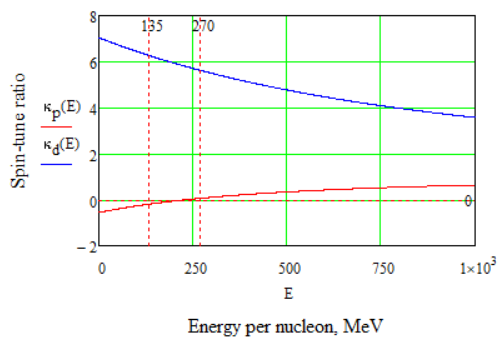
\includegraphics[width=0.6\linewidth]{4_spin-tune_ratio}
	\caption{Отношение спин-тюнов $\kappa = \cfrac{\nu_{\mathrm{B}_{\perp}}}{\nu_{\mathrm{E}}}$ поперечного магнитного и электрического поля для дейтрона и протона.}
	\label{fig:4_spin-tune}
\end{figure}

\par Эти фундаментальные различия приводят к нескольким важным выводам при построении структуры кольца. В частности, для изучения обоих типов частиц необходимо специальным образом проектировать установку. Согласно уравнению \ref{eq:deflection} направление вращения для протона и дейтрона различается. Это указывает на необходимость смены полярности полей спинового компенсатора, либо поворота его на $\pi$ вдоль продольной оси. Кроме того, минимально достижимая длина компенсатора определяемая уравнением \ref{eq:length_min}, для протона больше, чем для дейтронов при оптимальной энергии поляриметра. Это несоответствие может быть устранено путем снижения экспериментальной энергии для протонов (рис. \ref{fig:4_ele_length}). При длине спинового компенсатора, эквивалентной той, которая используется для дейтронов, энергия протонов должна быть снижена до 73 МэВ, анализирующая способность уменьшается в 2-3 раза, что полезно для проработки методики исследования, но недостаточно для статистической проверки (таблица \ref{tab:particles}). Двумя приемлемыми подходами для создания дополнительных электромагнитных полей в роли спинового компенсатора является применение фильтра Вина или электростатического дефлектора с кикером, что будет рассмотрено далее.

\begin{figure}[!h]
	\centering
	\includegraphics*[width=0.6\columnwidth]{4_total_length}
	\caption{Зависимость длины компенсирующего элемента в зависимости от энергии сгустка на нуклон.}
	\label{fig:4_ele_length}
\end{figure}

\begin{table}[!htb]
	\centering
	\caption{Параметры частиц и эксперимента.}
	\label{tab:particles}
	\begin{tabular}{lccccc}
		\toprule
		Частицы & $A/Z$ & $G$     & $\gamma_{\text{exp}}$ & $E_{\text{exp}}$, МэВ/нуклон  & $L$, м \\
		\midrule
		Дейтрон $\text{d}$ & $2$   & $-0.14$ & $1.144$  & $135$ & $53$ \\
		Протон $\text{p}$ & $1$   & $1.79$  & $1.289$ & $270$ & $247$ \\
		&    &   & $1.078$ & $73$ & $53$ \\
		\bottomrule
	\end{tabular}
\end{table}

	\subsection{Применение прямого фильтра Вина со скрещенными полями}

\par Фильтр Вина является важным инструментом в ускорителях частиц, предназначенным для манипуляции спиновой динамики без изменения орбитальной траектории частиц. Это достигается за счет использования перпендикулярных магнитного и электрического поля, которые компенсируют друг друга, что приводит также к компенсации силы Лоренца и не возмущает спин за счет ЭДМ. Такая конфигурация позволяет частицам двигаться по прямой линии, обеспечивая при этом компенсацию МДМ-эффекта, что делает фильтр идеальным для экспериментов, требующих манипуляций со спином. Конструкция фильтра гарантирует отсутствие чистого отклонения вдоль линии пучка, минимизируя дополнительные требования к пространству в прямых секциях кольца и предполагает классическое последовательное расположение элементов кольца.

\par На рис. \ref{fig:wien-filter} представлены принципиальные схемы квази-замороженного спина для дейтрона, так и для протона. Во-первых, показано, что отклонение спина за один период из-за МДМ-эффекта в магнитной арке значительно больше для протона. Во-вторых, направления полей для разного сорта частиц меняют знак.

\begin{figure} [h!]
	\centering
	а. Протон\\
	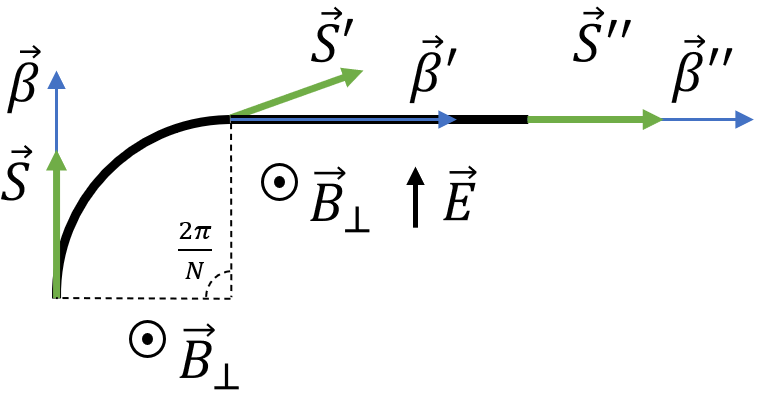
\includegraphics[width=0.6\linewidth]{4_wien-filter_deuteron}\\
	б. Дейтрон\\
	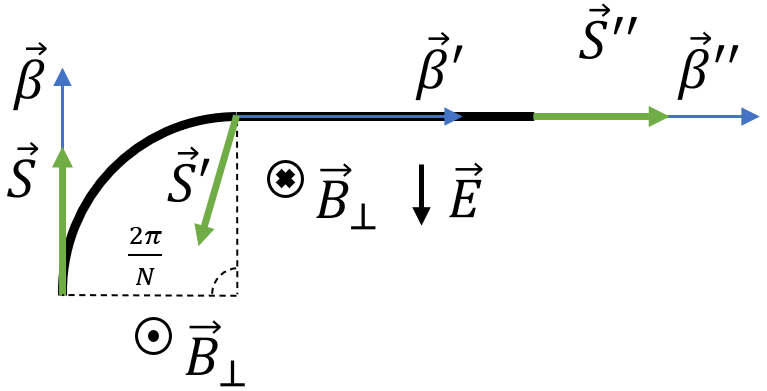
\includegraphics[width=0.6\linewidth]{4_wien-filter_proton}
	\caption{Принципиальная схема одного периода квази-замороженной структуры с фильтрами Вина для а. дейтронов, б. протонов.}
	\label{fig:wien-filter}
\end{figure}

\par Адаптивность фильтра Вина проявляется в возможности его использовании как для дейтронов, так и для протонов; для дейтронов он может быть использован непосредственно на оптимальных энергиях, тогда как для протонов в той же структуре необходимо изменить полярность или повернуть установку на $\pi$ вдоль продольной оси и использовать на более низких энергиях. Эта гибкость способствует разработке методологии для изучения спиновой динамики различных типов частиц, улучшая экспериментальные подходы. В целом, способность фильтра Вина управлять спином частиц без нарушения их орбиты, делает его перспективным элементом в современных прецизионных  экспериментах.

	\subsection{Применение электростатического дефлектора и дополнительного киккера}

\par Чисто электростатический дефлектор предназначен для изменения как траекторий частиц, так и спиновой динамики, при этом создается радиальное электрическое поле с ненулевой кривизной. В отличие от фильтра Вина, дефлектор требует дополнительного киккера для компенсации орбитальных отклонений, что увеличивает общую длину спинового компенсатора. 
\par При необходимости введения электростатической арки с кривизной $\Phi_{p\textrm{E}}^{\textrm{def}}$, магнитные арки должны дополнительно поворачивать на угол $\Phi_{p\textrm{B}}^{\textrm{kick}}$ при помощи киккеров. Такой поворот будет впоследствии скомпенсирован поворотом в электростатической арке. На рис. \ref{fig:4_arc_B_E}а изображено поведения спин-вектора для дейтрона при последовательном действии магнитной арки, киккера, электростатической арки с отрицательной кривизной и симметрично расположенного киккера. Для протона же меняется кривизна электростатической арки, а также дополнительных киккеров, а для измерений на полной энергии увеличивается и их эффективная длина, что показано на рис. \ref{fig:4_arc_B_E}б. Поворот импульса, после прохождения периода должен также быть повернуть на $\frac{2\pi}{N}$ для обеспечения квази-замороженного условия.

\begin{figure} [h!]
	\centering
	а. Дейтрон\\
	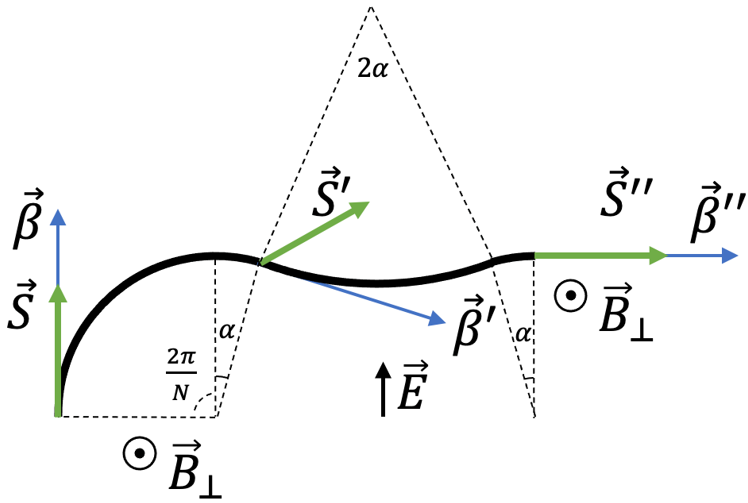
\includegraphics[width=0.6\columnwidth]{4_deflector_deutron}\\
	б. Протон\\
	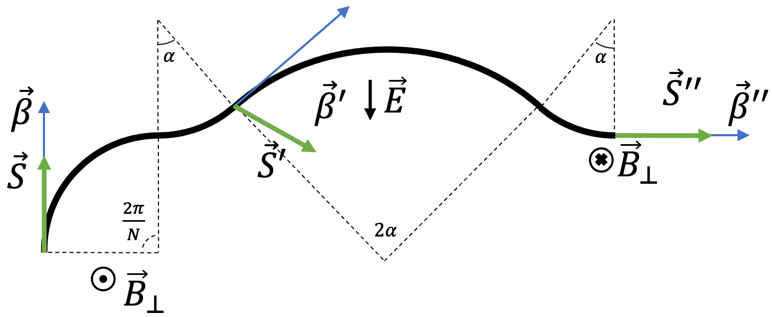
\includegraphics[width=0.77\linewidth]{4_deflector_proton}
	\caption{Принципиальная схема одного периода квази-замороженной структуры с электростатическими дефлекторами для а. дейтронов, б. протонов.}
	\label{fig:4_arc_B_E}
\end{figure}

\par Использование таких элементов особенно интересно для создания обходных секций в дополнение к исходным прямым секциям, позволяя варьировать структуру установки. Однако, необходимо учитывать расстояние между пространственным расположением оборудования, чтобы обеспечить возможность независимой работы. Основная сложность заключается в том, что для каждого типа частиц требуется различная кривизна, которую необходимо определить на этапе проектирования структуры. Несмотря на эти сложности, электростатический дефлектор с киккером предлагает надежное решение для управления спином и траекторией частиц.
\newline
\par Такой результат говорит о том, что принципиальным для реализации квази-замороженности остается наличие отклоняющих полей. При использовании чисто электростатических дефлекторов, необходимо использовать дополнительный внешний магнитный толчок. В случае же прямого фильтра Вина используется скрещенные магнитное и электростатическое поля. Интегральная величина поля при этом сохраняется.

\par  Как видно из рассмотренных принципиальных структур, изучение одновременно ЭДМ дейтрона и протона в структуре с электростатическими дефлекторами не целесообразно по сравнению со структурой с использованием фильтров Вина. Во-первых, требуемая длина дефлекторов равна длине фильтров Вина, но в первом случае необходимы дополнительные киккеры. Во-вторых, кривизна дефлекторов для протонов и дейтронов имеет различный знак. В тоже время, фильтры Вина устанавливаются на прямой участок и не требуют альтернативного канала. А для изучения протонов в фильтрах Вина может быть изменена полярность, либо сам элемент повернут на 180 градусов относительно продольной оси. Использование дефлекторов может быть полезно в случае естественной способности орбитально отклонять пучок, что позволяет создать альтернативный канал.

	\section{Применение концепции квази-замороженного спина в действующих ускорительных установках}\label{sec:EDM/nuclotron}

\par В настоящее время предложенные энергетические требования для ЭДМ исследований установлены на уровне 270 МэВ и ниже, однако никаких ограничений относительно орбитального вращения в арке не сделано. Основным условием является достижения поворота импульса на определенный угол $\Phi_p^{\textrm{arc}}$ с соответствующим поворотом $\Phi_s^{\textrm{arc}}$ для спина. Это может быть достигнуто путем достаточного набора интеграла магнитного поля в диполях. Величина магнитного поля может быть произвольной, чтобы добиться максимальной эффективности и минимизировать эффективную длину арки, поле должно быть максимально возможным, учитывая уникальные особенности структуры. Такой подход не только оптимизирует исследования на текущем уровне энергии, но и открывает возможности для других исследований поляризованных или неполяризованных пучков на более высоких энергиях, потенциально достигающих нескольких ГэВ. Универсальность квази-замороженной структуры позволяет внедрять её в различные установки, включая существующие ускорительные кольца, тем самым отвечая современным экспериментальным требованиям для работы на повышенных уровнях энергии. Применение изложенного подхода будет рассмотрено сразу для двух установок ОИЯИ: Nuclotron - являющемся бустером для коллайдера, так и самого коллайдера NICA. 

	\section{Использование Nuclotron в качестве бустера легких поляризованных частиц в коллайдер NICA}\label{sec:EDM/nuclotron}

\par Рассмотрим возможность использования синхротрона Nuclotron для ЭДМ исследований с применением концепции квази-замороженного спина.
\par В первую очередь, текущая структура Nuclotron предназначена для ускорения поляризованные протоны до энергии порядка $8$ ГэВ с возможной последующей инжекцией в коллайдер NICA для экспериментов на SPD детекторе при энергии $12.6$ ГэВ. Как было показано ранее в Главе \ref{ch:transition}, прохождение критической энергии без потерь в регулярной структуре коллайдера NICA при энергии $5.7$ ГэВ для протонного поляризованного пучка является необходимым требованием эксперимента для достижения требуемой светимости. Таким образом, могут быть рассмотрены 2 вариации инжекции из бустера 1) ниже критической; 2) выше критической энергии коллайдера NICA. В первом случае, необходимо осуществить скачок критической энергии непосредственно в кольце коллайдера, что накладываются существенные ограничения на параметры пучка, в результате которых снижается светимость конечного эксперимента. Во втором случае, после инжекции необходимо охлаждение пучка при энергии 7-10 ГэВ. Однако, текущий электронный охладитель рассчитан на энергию пучка 2-3 ГэВ, что делает необходимым разработку новой установки электронного охлаждения на повышенной энергии.

\par Альтернативно, в Главе \ref{ch:resonant} был представлен вариант модернизации модернизация кольца NICA с повышенной критической энергией. При таком подходе проблем с прохождением критической энергии не возникает, поскольку во всем диапазоне энергий вплоть до конечной энергии эксперимента критическая энергия не преодолевается вовсе. В этом случае инжекция может осуществляться на энергии $2-3$ ГэВ с эффективным электронным охлаждением на уже разработанной установке. Таким образом, максимальная энергия кольца Nuclotron может быть снижена без потери функции бустера.

	\subsection{Требования к магнитооптической структуре синхротронов Nuclotron-NICA в задаче исследования электрического дипольного момента легких ядер}\label{sec:EDM/requirements}

Окончательно, сформулируем ключевые требования, которые должны быть реализованы при модернизации кольца Nuclotron:

\begin{enumerate}
    \item Использование Nuclotron в качестве бустера поляризованных частиц в коллайдер NICA при минимальной энергии протонного пучка 2-3 ГэВ;
    \item Возможность проведения прецизионных экспериментов по исследованию ЭДМ заряженных частиц с использованием квази-замороженной концепции.
\end{enumerate}

\par Текущая структура Nuclotron не предполагает проведения экспериментов по исследованию ЭДМ. Рассмотрим возможные способы реализации такой программы как на текущей установке, так и возможные опции по модернизации. В первую очередь, рассмотрим необходимые требования с точке зрения спиновой динамики. Основным является требование скомпенсированности МДМ компоненты. Для достижения этого эффекта может быть использован метод замороженного спина, в этом случае МДМ вращение равняется нулю для всего кольца. При таком подходе спин остается с всюду со-направлен с направлением импульса. Как можно увидеть из уравнений Т-БМТ и проведенного ранее анализа, необходимо использование элементов со скрещенными магнитными и электрическим полями. Наличие чисто магнитных арок приводит к невозможности использовать метод замороженного спина для компенсации МДМ вращения спина.

\par И как было показано, альтернативным является метод квази-замороженного спина, в отличие от замороженного спина предполагает пространственное разделение электрического и магнитных полей и последовательная компенсация МДМ-компоненты. Компенсация может быть осуществлена на прямых участках с необходимостью использовать электрическое поле. Для текущей опции могут быть рассмотрены как чисто электростатические дефлекторы, так и фильтры Вина с перпендикулярными электрическим и магнитным полем.

\par Стоит отметить, что поскольку Nuclotron должен быть использован в качестве бустера в NICA, то необходимо реализовать структуру, работающую для ускорения поляризованного протонного пучка до энергии порядка единицы ГэВ, и одновременно с этим низкоэнергетическую опцию при энергии порядка сотен МэВ с возможностью изучения ЭДМ. Таким образом, ведущим полем должно выступать магнитное поле в поворотных магнитах, поскольку электрическое поле неспособно ускорить до энергии порядка единиц ГэВ. Кроме того, отдельное внимание будет уделено критической энергии Нуклотрона. Она должна лежать выше максимальной энергии пучка для сохранения его стабильности.
	
	\subsection{Текущая магнитооптика Nuclotron}\label{sec:EDM/optics}
\par Принципиальная схема текущей восьмипериодической структуры Nuclotron с длиной $L_{\text{NUC}}=251$ м. представлена на рис. \ref{fig:4_Nuclotron_original}а. На рис.\ref{fig:4_old_nuclotron} изображены параметры Твисса для одного периода, неоптимальные с точки зрения подавления дисперсионной функции на прямых участках. Суммарная длина прямых промежутков составляет $L_{\text{free}} = 7\times8=56$ и в немодернизированной структуре Нуклотрона, расположение фильтров Вина с длиной $L_{\text{WF}} = 53$ м. полностью займёт всё пространство на прямых участках без возможности использования другого необходимого оборудования. Поэтому, рассмотрим возможность создания обходных каналов в исходной структуре. При таком подходе, оборудование можно расположить параллельно при наличии достаточного расстояния между полученными каналами. На рис. \ref{fig:4_Nuclotron_original}б показана принципиальная схема текущей структуры Nuclotron с электростатическими дефлекторами. Максимальное расстояние между каналами может составить порядка $18$ см, чего недостаточно для параллельного расположения.

\begin{figure}[!h]
	\centering
	а.\includegraphics*[width=0.47\columnwidth]{4_Nuclotron_original.png}
	б.\includegraphics*[width=0.47\columnwidth]{4_Nuclotron_original_def.png}
	\caption{Принципиальная схема расстановки структуры Nuclotron с текущей расстановкой элементов и с введением электростатических дефлекторов.}
	\label{fig:4_Nuclotron_original}
\end{figure}

\begin{figure}[!h]
  \centering
	\includegraphics*[width=0.99\columnwidth]{4_old_nuclotron}
   \caption{Твисс-функции текущей регулярной структуры Nuclotron.}
   \label{fig:4_old_nuclotron}
\end{figure}

\par Приведенные факты показывают необходимость модернизации для увеличения длины прямых участков, может быть рассмотрена модернизация с оптимизацией диполей с магнитным полем $1.8$ Тл. Суммарная длина прямых промежутков должна составить $L_{\text{free}}+L_{\text{WF}}=56+53 = 109$ м. Оставшееся место будет использовано для расстановки магнитных элементов, диполей, квадруполей, секступолей. Длина магнитной арки $L_{\textrm{arc}}=17.5$ м, а длина магнитов изменяется от $1.44$ м. до $1.78$ м., при этом их количество сокращается вдвое с $96$ до $48$. Тогда максимальная энергия протонного пучка может максимально составлять $6.5$ ГэВ. Данная опция, удовлетворяет требованию использования Nuclotron в качестве бустера при $2-3$ ГэВ, а также возможности его использования на выведенной мишени экспериментов BM@N c понижением энергии от $10$ ГэВ до $6.5$ ГэВ \cite{kovalenko:nuclotron}. В случае фильтров Вина – они могут быть расположены в этом же канале последовательно, а для дефлекторов неизбежно должны быть реализованы дополнительные каналы.

	\subsection{Модернизированная восьмипериодическая структура}\label{sec:EDM/optics/8period}

\par С учетом вышесказанного, была реализована восьмипериодическая структура на основе простейшей ФОДО ячейки. В такой структуре может быть применены обе опции подавления МДМ-компоненты: прямыми фильтрами Вина и электростатическами дефлекторами с киккер-магнитами.

\par В этом случае интересным является случай с использованием дефлекторов, тогда нет необходимости использовать прямые промежутки для нужд ЭДМ эксперимента. Дефлекторы могут быть расставлены как по краям, так и в центре рис. \ref{fig:4_Nuclotron_8}, при этом расстояние между каналами составляет $47$ и $50$ см соответственно.

\par Подавление дисперсии на арки может быть осуществлено выбором кратного количества набега фазы $\nu_{x,y} = 1$, что показано на рис. \ref{fig:4_Nuclotron_8}. Стоит отметить, что наличие электростатики при энергии $E_{\textrm{edm}}=270$ МэВ, искажает дисперсию на длине периода, которая не компенсируется соответствующим магнитным полем. Однако, она может быть дополнительно компенсирована квадруполями арки, при этом набег фазы также искажается, что может приводить к сложностям с подавлением нелинейности. Пример такой компенсации показан на рис. \ref{fig:4_Nuclotron_twiss_8}.

\begin{figure}[!h]
  \centering
   \includegraphics*[width=0.49\columnwidth]{4_Nuclotron_8_def1.png}
   \includegraphics*[width=0.49\columnwidth]{4_Nuclotron_8_def2.png}
   \caption{Принципиальная схема расстановки восьмипериодической структуры Nuclotron с текущей расстановкой при введении электростатических дефлекторов.}
   \label{fig:4_Nuclotron_8}
\end{figure}

\begin{figure}[!h]
  \centering
   \includegraphics*[width=1\columnwidth]{4_Nuclotron_twiss_8}
   \caption{Твисс-функции регулярной поворотной арки восьмипериодической модернизированной структуры Nuclotron.}
   \label{fig:4_Nuclotron_twiss_8}
\end{figure}

\begin{figure}[!h]
  \centering
   \includegraphics*[width=1\columnwidth]{4_Nuclotron_Def_twiss_8}
   \caption{Твисс-функции регулярной поворотной арки восьмипериодической модернизированной структуры Nuclotron с дефлекторами.}
   \label{fig:4_Nuclotron_Def_twiss_8}
\end{figure}

\newpage
	\subsection{Модернизированная 16-периодическая структура}\label{sec:EDM/optics/16period}

\begin{figure}[!h]
  \centering
   \includegraphics*[width=0.5\columnwidth]{4_Nuclotron_16.png}
   \caption{Принципиальная схема расстановки восьмипериодической структуры Nuclotron с текущей расстановкой при введении электростатических дефлекторов.}
   \label{fig:4_Nuclotron_16}
\end{figure}

\begin{figure}[!h]
  \centering
   \includegraphics*[width=1\columnwidth]{4_Nuclotron_twiss_16.png}
   \caption{Твисс-функции 16-периодической модернизированной структуры Nuclotron без фильтров Вина.}
   \label{fig:4_Nuclotron_twiss_16}
\end{figure}

\begin{figure}[!h]
  \centering
   \includegraphics*[width=1\columnwidth]{4_Nuclotron_WF_twiss_16.png}
   \caption{Твисс-функции 16-периодической модернизированной структуры Nuclotron c фильтрами Вина.}
   \label{fig:4_Nuclotron_twiss_16}
\end{figure}

\par С целью увеличения точности проведения эксперимента, квази-замороженный спин может быть как можно больше приближен к режиму замороженного спина при увеличении периодичности, согласно ур. \ref{eq:edm}. Особенно это важно для изучения ЭДМ протона, согласно таблице \ref{tab:edm}. Для этого, в уже рассмотренном случае восьмипериодической структуры, магнитная арка может быть раздвинута для создания дополнительного прямого промежутка, однако такой подход нарушает регулярность и соответствующая структура должна быть рассмотрена как резонансная, подобно представленному в Главе \ref{ch:resonant}. Стоит отметить, что 16-ти периодической эта структура называется именно по причине возможности разделения фильтров Вина на большее количество, делая угол отклонения спина меньше двое, по сравнению с приведенной выше структурой. Однако, по своей сути, магнитная структура имеет периодичность равную 8.

\par С точки зрения построения магнито-оптической структуры модернизированного Нуклотрона следовали нескольким целям. Во-первых, как мы видим суперпериод построен таким образом, чтобы в центральной ячейке было дрейфовое пространство без поворотных магнитов, в том месте, где дисперсионная функция имеет максимальное значение при бесконечном значении кривизны траектории, что позволит поднять критическую энергию. Во-вторых, число суперпериодов равное восьми, незначительно превышает частоту бетатронных колебаний ${\nu}_x$ в горизонтальной плоскости, что облегчает регулировку коэффициента уплотнения орбиты. В-третьих, введение центрального дрейфа упрощает размещение трех семейств секступолей, необходимых для регулирования бетатронной и спиновой хроматичностей, в то время, как боковые дрейфовые участки удобны для размещения фильтров Вина.

\begin{table}[!htb]
	\centering
	\caption{Параметры структур Nuclotron.}
	\label{tab:structures}
	\begin{tabular}{|>{\raggedright\arraybackslash}p{2.7cm}|c|c|c|c|c|}
		\hline
		Структура & \makecell[c]{Длина \\ магнита, м} & \makecell[c]{Количество \\ магнитов} & \makecell[c]{$B\rho$, \\ Т$\cdot$м} & \makecell[c]{Макс. энергия \\ дейтронов, ГэВ} & \makecell[c]{Макс. энергия \\ протонов, ГэВ} \\
		\hline
		Текущая & 1.44 & 96 & 39.6 & 10.14 & 10.97 \\
		\hline
		8-период. & 1.78 & 48 & 24.4 & 5.7 & 6.47 \\
		\hline
		16-период. & 1.78 & 48 & 24.5 & 5.7 & 6.47 \\
		\hline
	\end{tabular}
\end{table}

	\section{Предпосылки модернизации главного кольца NICA}\label{sec:EDM/Wien_filter/modernization}

\par Для изучения ЭДМ в кольце коллайдера NICA рассматривается использование концепции квази-замороженного спина, поскольку поворотные арки являются чисто магнитными. Коллайдерная мода использует всё пространство прямых промежутков для установки необходимого оборудования (охлаждение, ускоряющие ВЧ-станции, диагностика), а также имеет точки соударения для изучения в детекторах. Для решения обоих указанных проблем, могут быть созданы альтернативные обводные каналы (bypass), в которых будут расположены прямые фильтры Вина. Таким образом, появляется возможность использования главного кольца NICA в качестве накопителя, а не в режиме коллайдера. Создание обводных каналов является большим преимуществом, не требующим значительной перестройки комплекса и затрат, при этом, позволяющим задействовать NICA в различных экспериментах. Особая форма коллайдера -- рейстрек (racetrack), состоит из двух магнитных поворотных арок и имеет таким образом периодичность равную двойке. Данная особенность существенно ограничивает потенциал установки для изучения ЭДМ протона, поскольку в такой конфигурации невозможно накопления ЭДМ-компоненты. Однако, сохраняется потенциал для изучения ЭДМ дейтрона. Отдельным преимуществом коллайдера является наличие двух колец и возможности изучения пучка в прямом и обратном направлении. Данное условие необходимо ЭДМ исследований.

\par Проектируя накопительное кольцо NICA с обводными секциями, требуется оставить геометрию арок неизменной для полного сохранения исходных функций. Возможно лишь изменение полей в уже установленных элементах. В будущем вся предлагаемая магнитооптика будет рассмотрена для дейтронов с энергией $240$ МэВ. Стоит отметить, что расчеты показывают основные параметры магнитного поля основных диполей арки $B_{\textrm{dip}}=0.132$ Т, а также магнитную жесткость $B\rho=3.252 \ \textrm{T} \cdot$м. Ненулевая дисперсия в поворотной арке подавлена по краям, таким образом прямой участок имеет нулевую дисперсию по всему периметру. Общая длина оригинального кольца NICA $L_{\textrm{acc}}=503.04$ м., длина одной арки составляет $L_{\textrm{arc}}=142.15$ м., остаётся доступным $\left(L_{\textrm{acc}}-2L_{\textrm{arc}}\right)/2=109.6$ м. для организации обводного канала.

\par Для орбитального отклонения рассматривались дипольные магниты, чтобы обеспечить отклонение на угол $\alpha=\ 9$. Сила диполя $B_{\textrm{BP}}=1$ Т при длине $L_{\textrm{dip}}^{\textrm{BP}}=50$ см. Альтернативный прямой участок находится на расстоянии $1$ м от исходного, поэтому длина обводного участка $L_{\textrm{BP}}=1\mathrm{м/sin\alpha}\sim6.4$ м. Принципиальная схема обходных каналов показана на рисунке \ref{fig:4_NICA_bypass}.

\begin{figure}[!h]
  \centering
   \includegraphics*[width=1.0\columnwidth]{4_NICA_bypass.png}
   \caption{Принципиальная схема обходных каналов bypass в существующем комплексе NICA.}
   \label{fig:4_NICA_bypass}
\end{figure}

\par Отклоняющие магниты искажают дисперсионную функцию. Таким образом, необходимо было использовать по меньшей мере 2 фокусирующих квадруполя на обходном канале для подавления дисперсия на выходе. Это поможет обеспечить нулевую дисперсию на всем прямолинейном участке. Чтобы гарантировать периодичность и симметрию бета-функций, можно использовать или один, или три дефокусирующих квадруполя. Будут рассмотрены два случая, с адаптированными прямыми участками, идентичным поворотным аркам, но без магнитов. Это сделано для простоты моделирования в регулярной идеальной структуре. Наконец, мы рассмотрим реальный случай магнитооптики с полностью регулярной ФОДО прямой секцией.

	\subsection{Первичная схема с 3 квадруполями}\label{sec:EDM/Wien_filter/ByPass/3quad}

\par В этом случае байпас состоит из минимально возможных 3 квадруполей: 2 фокусирующих QBP1 и 1 дефокусирующий QBP2, что показано на рис. \ref{fig:4_bypass_3scheme}. Согласование арки с каналом bypasss обеспечивается тремя квадруполями QM1, QM2, QM3 (секция согласователя Matching M1). А согласование bypass с прямым участком симметрично осуществляется такими же квадруполями QM1, QM2, QM3. Это возможно в силу изначально заложенной симметрии между аркой и прямым участком. Тогда общая длина всего ускорителя составит $L_{\textrm{3quad}}^{\textrm{acc}}=503.46$ м.
\par На рисунке \ref{fig:4_bypass_3quad} приведены Твисс-функции, черными линиями указаны границы отклоняющего участка. Максимум бета-функции $\beta_y$ расположен в центре канала. И может принимать большее значение, по сравнению с $\beta_{x}$. По этой причине можно рассмотреть случай с 5 квадруполями в обводном канале.

\begin{figure}[!h]
  \centering
   \includegraphics*[width=1.0\columnwidth]{4_bypass_3scheme.png}
   \caption{Принципиальная схема bypass с 3 квадруполями.}
   \label{fig:4_bypass_3scheme}
\end{figure}

\begin{figure}[!h]
  \centering
   \includegraphics*[width=1.0\columnwidth]{4_bypass_3quad}
   \caption{Твисс-параметры для bypass с 3 квадруполями. Черными линиями показано расположение дефлекторов.}
   \label{fig:4_bypass_3quad}
\end{figure}

	\subsection{Модернизированная схема с 5 квадруполями}\label{sec:EDM/Wien_filter/ByPass/5quad}

\par По сравнению с предыдущим случаем, обводной канал состоит из 5 квадруполей, которые представлены 2 семействами: фокусирующим QBP1 и дефокусирующим QBP2. Он становится длиннее $L_{\textrm{5quad}}^{\textrm{BP}}=9.35$ м и отклоняется на $1.46$ м., что показано на рис. \ref{fig:4_bypass_5scheme}. Теперь секции согласования M1 и M2 по-прежнему идентичны, но представлены двумя квадруполями QM1 и QM2 для обеспечения регулярности Твисс-функций. Однако, полная длина ускорителя становится больше исходного $L_{\textrm{5quad}}^{\textrm{acc}}=510.02$ м. На рисунке \ref{fig:4_bypass_5quad} показаны, что максимум $\beta_y$ становится меньше в центре. Стоит отметить, что максимум дисперсионной функции стал увеличился от $D_x^{\textrm{3quad}} \sim 0.2$ м до $D_x^{\textrm{5quad}} \sim 0.5$ м. Таким образом, этот случай должен быть адаптирован к реальному.

\begin{figure}[!h]
  \centering
   \includegraphics*[width=1.0\columnwidth]{4_bypass_5scheme.png}
   \caption{Принципиальная схема bypass с 5 квадруполями.}
   \label{fig:4_bypass_5scheme}
\end{figure}

\begin{figure}[!h]
  \centering
   \includegraphics*[width=1.0\columnwidth]{4_bypass_5quad}
   \caption{Твисс-параметры для bypass с 5 квадруполями. Черными линиями показано расположение дефлекторов.}
   \label{fig:4_bypass_5quad}
\end{figure}

	\subsection{Адаптированный вариант}\label{sec:EDM/Wien_filter/ByPass/final}

\par Основываясь на рассмотренных примерах, наконец, можно получить структуру, максимально адаптированную к реальным длинам установки. Теперь рассмотрим полностью регулярный прямой участок, который стал короче $L_{\textrm{SS}}^{\textrm{BP}}=80.71$ м (рис. \ref{fig:4_bypass_real_scheme}). Отклоняющий канал состоит из 5 квадруполей и отклоняет пучок на $1.46$ м. Но для согласования использовались разные секции M1 и M2, чтобы компенсировать асимметрию между поворотной аркой и прямым участком. Наконец, Твисс-функция половины bypass NICA, представлена на рисунке \ref{fig:4_bypass_twiss_ring}. В центре прямой секции расположены фильтры Вина. Все расчеты выполнены при помощи программ OptiM \cite{optim} и COSY Infinity \cite{cosy}.

\begin{figure}[!h]
  \centering
   \includegraphics*[width=1.0\columnwidth]{4_bypass_real_scheme.png}
   \caption{Принципиальная схема адаптированной структуры кольца NICA c bypass.}
   \label{fig:4_bypass_real_scheme}
\end{figure}

\begin{figure}[!h]
  \centering
   \includegraphics*[width=1.0\columnwidth]{4_bypass_twiss_ring.png}
   \caption{Твисс-функции для половины адаптированной структуры кольца NICA c bypass. Фильтры Вина, расположенные на прямом участке.}
   \label{fig:4_bypass_twiss_ring}
\end{figure}

\newpage
	
	\section{Cпин-орбитальный трекинг в магнитном кольце со скрещенными E+B элементами} \label{sec:EDM/Wien_filter_tracking}

\par Траектория спина показана на рисунке \ref{fig:4bypassspin} в одной половине модернизированного кольца bypass NICA и состоит из: поворотной арки, отклоняющего канала, прямого сегмента и двух секций согласователя (M1 и M2). Рассматривается вертикально поляризованная частица с небольшим начальным отклонением. Как видно, фильтры Вина на прямом участке компенсируют вращение спина в дуге и восстанавливают его до исходного значения.

\begin{figure}[!h]
	\centering
	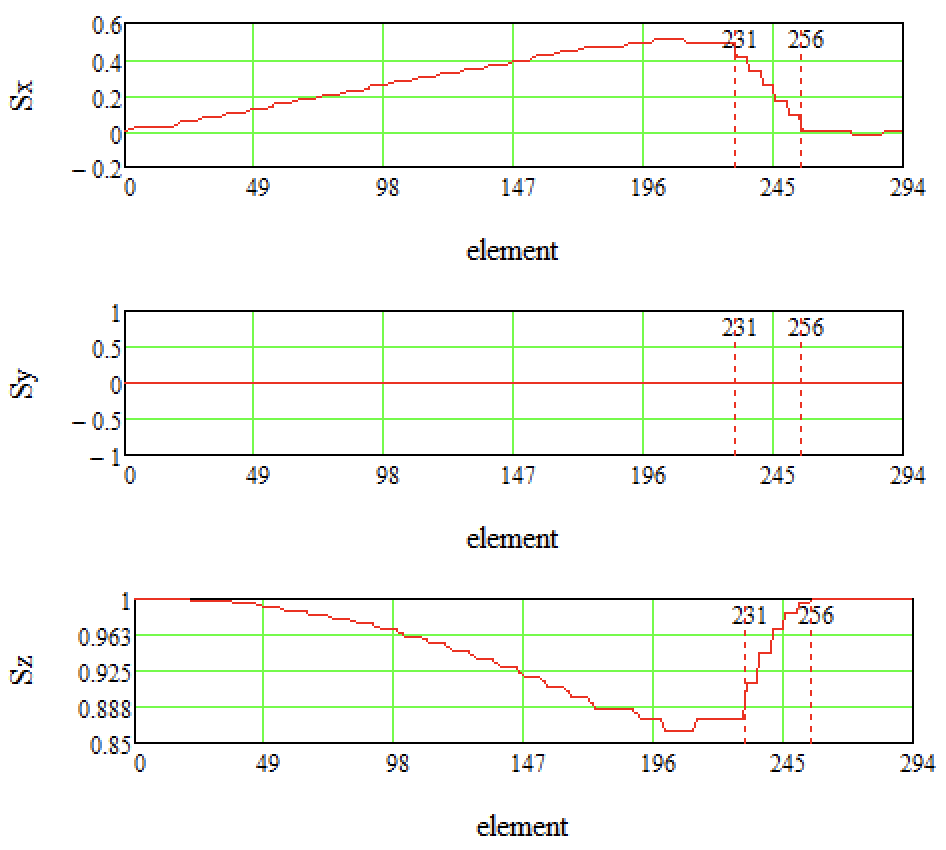
\includegraphics[width=0.7\linewidth]{images/4_bypass_spin}
	\caption{Траектория спина в половине модернизированного кольца bypass NICA. Арка и прямая секция с фильтрами Вина ((обозначены красными пунктирными линиями). Вертикально поляризованная частица $\vec{S}~(0,0,1)$. Показана зависимость $S_{x}$, $S_{y}$ и $S_{z}$ от номера элемента (длины).}
	\label{fig:4bypassspin}
\end{figure}

\par Орбитальное движение частиц в трехмерном пространстве оказывает влияние на спиновую динамику, и согласно ур. \ref{eq:T-BMT} спин различных частиц, прецессирует с отличными частотами вокруг инвариантной оси. При значительном разбросе, нарушается спиновая когерентность, тем самым ограничивая возможность измерения ЭДМ. Для обеспечения спиновой когерентности необходимо использовать нелинейные элементы, секступоли, расположенные в местах с ненулевой дисперсией, на поворотных арках. Так как секступоли также влияют и на бетатронную хроматичность, мы рассматриваем возможность одновременного подавления обоих эффектов.

		\subsection{Декогеренция спина}\label{sec:EDM/Wien_filter_tracking/decoherence}

\par Сдвиг распределения равновесного уровня энергии из-за бетатронного движения и ненулевого коэффициента уплотнения импульса второго порядка основан на синхронном принципе \cite{Senichev:2013_decoherence} и определяется с помощью:

\begin{equation}
\Delta\delta_{eq}=\frac{\gamma_s^2}{\gamma_s^2\alpha_0-1}\left[\frac{\delta_0^2}{2}\left(\alpha_1+\frac{3}{2}\frac{\beta_s^2}{\gamma_s^2}-\frac{\alpha_0}{\gamma_s^2}+\frac{1}{\gamma_s^4}\right)+\left(\frac{\Delta L}{L}\right)_\beta\right]
\label{eq:equilibrium}
\end{equation}

\noindent для определения относительного удлинения орбиты из-за бетатронных колебаний:

\begin{equation}
\left(\frac{\Delta L}{L}\right)_\beta=\frac{\pi}{2L}\left[\epsilon_x\nu_x+\epsilon_y\nu_y\right],
\end{equation}

\noindent где индекс $s$ означает синхронную частицу, $\epsilon_x$, $\epsilon_y$ – эмиттансы, $\nu_x$, $\nu_y$ – частота бетатронных колебаний, $\delta_0$ – относительный разброс импульса, $\alpha_0$, $\alpha_1$ – два первых порядка коэффициента уплотнения импульса. Разные частицы имеют различный импульс, и существует необходимость в использовании понятия эффективной энергии пучка:

\begin{equation}
	\gamma_{\text{eff}}=\gamma_s+\beta_s^2\gamma_s\Delta\delta_{eq}
\end{equation}

\par Более формальная теория подразумевает воздействие внешнего (секступольного) поля. Принимая во внимание выражение для полного удлинения орбиты из \cite{orbit_length}:

\begin{equation}
\Delta C_\Sigma=-2\pi\left(J_x\xi_x+J_y\xi_y\right)+\delta_0\left(\alpha_0+\alpha_1\delta_0+\alpha_2\delta_0^2+\ldots\right),
\label{eq:orbit_length}
\end{equation}

\noindent где $\xi_x$, $\xi_y$ – хроматичность в $x, y$ плоскостях. Исходя из представленных уравнений, для коррекции орбитального движения могут быть использованы секступоли для компенсации натуральной хроматичности, а также коэффициента уплотнения орбиты.

		\subsection{Секступольная коррекция}\label{sec:EDM/Wien_filter_tracking/sextupole_correction}

\par Достижение спиновой когерентности является отдельной сложной задачей, и такие эксперименты были проведены на ускорителе COSY в Юлихе, Германия, чтобы получить время когерентности (Spin Coherence Time) SCT на уровне $1000$ секунд \cite{1000}. Секступоли располагаются в местах с ненулевой дисперсией на поворотных арках. В минимумах и максимумах дисперсионной $D_{x,y}$ и бета $\beta_{x,y}$ функциях оказывают наибольшее воздействие и физически располагаются рядом с квадрупольными линзами. Твисс-функции арки NICA являются регулярными и показаны на рис. \ref{fig:4_NICA_arc}.

\begin{figure}[!h]
  \centering
   \includegraphics*[width=1.0\columnwidth]{4_NICA_arc.png}
   \caption{Твисс-параметры bypass NICA для дейтронного режима в OptiM. Также показано расположение секступольных семейств.}
   \label{fig:4_NICA_arc}
\end{figure}

\textbf{Бетатронная хроматичность}.
Для коррекции бетатронной хроматичности достаточно использовать только 2 семейства секступолей: одно вблизи фокусирующих квадруполей, другое – рядом с дефокусирующими. Натуральная хроматичность рассматриваемого накопительного кольца bypass NICA равна $\nu_{x,y}=-17/-17$. После оптимизации можно отслеживать частоту прецессии спина на рис. \ref{fig:4_spin_dependance}: красная линия показывает натуральную хроматичность, синяя – скорректированную, подавленную до нуля. Для этого случая также был осуществлен спин-трекинг в течение $3\times{10}^6$ оборотов для частиц с различным начальным отклонением в координатах $x, y, d$ с начальной ориентацией спина ${\vec{S}}_0$ под углом $45$ градусов в плоскости $y-z$, что показано на рис. \ref{fig:4_spin_decoherence}.

\begin{figure}[!h]
	\centering
	\includegraphics*[width=0.32\columnwidth]{4_spin_dependance_x.png}
	\includegraphics*[width=0.32\columnwidth]{4_spin_dependance_y.png}
	\includegraphics*[width=0.32\columnwidth]{4_spin_dependance_d.png}
	\caption{Зависимость частоты прецессии спина от координат x, y, d для различных случаев оптимизации. NC – натуральная хроматичность (красная линия); BC – нулевая (бетатронная) хроматичность (синяя пунктирная линия); SC – спиновая когерентность (зеленая линия); $BC_{\alpha}$ – нулевая хроматичность и $\alpha_1=0$ (фиолетовая линия); $BC_{\text{eta}}$ – нулевая хроматичность и ноль $\eta_1=0$ (светло-голубая линия).}
	\label{fig:4_spin_dependance}
\end{figure}

\begin{figure}[!h]
  \centering
   \includegraphics*[width=0.7\columnwidth]{4_spin_decoherence.png}
   \caption{Спиновый трекинг частиц с различным начальным отклонением в координатах x, y, d с использованием 2 семейств секступолей для получения нулевой бетатронной хроматичности.}
   \label{fig:4_spin_decoherence}
\end{figure}

\textbf{Спиновая когерентность}. Чтобы достигнуть спиновой когерентности, рассмотрим чисто частоту прецессии спина. COSY Infinity \cite{cosy} не может работать вблизи нулевого значения частоты прецессии спина. Так как это может привести к ошибке из-за резонанса, по этой причине отстраиваемся до уровня $\nu_s\sim{10}^{-4}$. Но к частицам предъявляется требование прецессировать синхронно — когерентно. Основным параметром является частота вращения спина, которая в общем случае зависит от координат и энергии. Можно видеть, что доминирующим компонентом является квадратичный член в разложении частоты спиновой прецессии. Это видно на Рисунке 2 для обоих случаев – как для натуральной хроматичности, так и скорректированной хроматичности. По этой причине секступоли могут быть выбраны другим способом, чтобы достигнуть спиновой когерентности, путем подавления вторых порядков.

\par Как мы можем видеть из ур. \ref{eq:equilibrium}, \ref{eq:orbit_length} недостаточно использовать только 2 линейно независимых семейства для независимой вариации трёх параметров орбитального движения. Таким образом, третье семейство должно быть использовано для подавления зависимости от энергетической компоненты. Но в регулярных структурах бета $\beta$ и дисперсионные $D$ функции не позволяют использовать 3 линейных независимых семейства. Введение линейно-зависимых семейств показано на параметрах Твисса, где расположены семейства: SF1, SF2, SD. В этом методе мы не влияем на хроматичность, просто отслеживаем её значение $\nu_{x,y}=-13/-18$. Этого недостаточно для обеспечения стабильного орбитального движения. В этом случае можно видеть, что спиновая когерентность достигнута -- нет зависимости частоты спиновой прецессии от координат и энергии (рис. \ref{fig:4_spin_dependance}: зеленая линия). Результаты спинового трекинга частиц подтверждают это утверждение. На рис. \ref{fig:4_spin_coherence}, частота вращения спина $\nu_s~{10}^{-7}$, количество оборотов $3\times{10}^6$ оборотов или $3$ секунды. Частицы с различным начальным отклонением прецессируют с одинаковой спиновой частотой. Но в этом случае максимум секступольного коэффициента принимает большое значение, что может вызвать нелинейные эффекты (Таблица \ref{tab:coherence}).

\begin{figure}[!h]
  \centering
   \includegraphics*[width=0.7\columnwidth]{4_spin_coherence.png}
   \caption{Спиновый трексинг частиц с различным начальным отклонением в координатах x, y, d с использованием 3 семейств секступолей для получения спиновой когерентности.}
   \label{fig:4_spin_coherence}
\end{figure}

		\subsection{Коррекция высших порядков}\label{sec:EDM/Wien_filter_tracking/correction}

\begin{table}[!hb]
	\centering
	\caption{Сравнение параметров с различной вариацией оптимизации оптимизацией.}
	\begin{tabular}{|p{2.6cm}|m{2.5cm}|m{2.5cm}|m{2.5cm}|m{2.5cm}|m{2.5cm}|}
		\hline
		Параметр & Без оптимизации & Хро\-ма\-тич\-ность & Спиновая когерентность & Хро\-ма\-тич\-ность + $\alpha_1$ & Хро\-ма\-тич\-ность + $\eta_1$ \\
		\hline
		Значение хроматичности & -17/-17 & 0/0 & -13/-18 & 0/0 & 0/0 \\
		\hline
		Коэф. $\alpha_1$ & 0.2 & -0.4 & $-0.37 \times 10^{-2}$ & $\sim -10^{-12}$ & -0.85 \\
		\hline
		Коэф. $\abs{K_x}$ & $0.16 \times 10^{-1}$ & $0.55 \times 10^{-1}$ & $0.27 \times 10^{-13}$ & $0.55 \times 10^{-1}$ & $0.56 \times 10^{-1}$ \\
		\hline
		Коэф. $\abs{K_y}$ & $0.51 \times 10^{-2}$ & $0.76 \times 10^{-1}$ & $0.12 \times 10^{-12}$ & $0.78 \times 10^{-1}$ & $0.78 \times 10^{-1}$ \\
		\hline
		Коэф. $\abs{K_z}$ & $0.43 \times 10^{-1}$ & $0.20 \times 10^{-1}$ & $0.13 \times 10^{-12}$ & $0.13 \times 10^{-1}$ & $1.6 \times 10^{-1}$ \\
		\hline
		\# семейств секступолей & Без секступолей & 2 & 3 & 3 & 3 \\
		\hline
		Макс. поле секступолей [m$^{-3}$] & - & 2.7 & 19.4 & 4.9 & 104.2 \\
		\hline
	\end{tabular}
	\label{tab:coherence}
\end{table}

\par Как мы можем видеть, чистая коррекция бетатронной хроматичности не позволила нам получить нулевой разброс частоты вращения спина. Одновременно, получение спиновой когерентности, путем подавления квадратичного члена частоты спиновой прецессии, не подавляет хроматичность. Исходя из ур. \ref{eq:orbit_length}, значение $\delta_0\alpha_0$ может быть усреднено с использованием ВЧ для смешивания. Таким образом, чтобы гарантировать нулевое удлинение орбиты, хроматичности должны быть подавлены $\xi_x,\xi_y$ вместе со значением $\alpha_0$ до нуля. Это также возможно при использовании только независимых 3-х семейств секступолей. Представленный способ не позволяет добиться спиновой когерентности в представленной структуре. На рис. \ref{fig:4_spin_dependance} (фиолетовая линия) показана ненулевая зависимость частоты прецессии спина от координат. Аналогичное справедливо, если мы следуем ур. \ref{eq:equilibrium} и подавляем значение $\eta_1$ вместе с коррекцией хроматичности (рис. \ref{fig:4_spin_dependance} светло-синяя линия). Кроме того, максимальное значение секступольного градиента слишком велико и не может быть реализовано.

\par Окончательно, были рассмотрены различные случаи оптимизации секступолями. Квадратичные члены в разложении по частоте спиновой прецессии являются наиболее важными и представляют зависимость от координат и энергии. Все основные параметры, которые подвергались мониторингу, приведены в Таблице \ref{tab:coherence}. Исследование показывает, что невозможно использовать 3 семейства секступолей в регулярной структуре для достижения как бетатронной хроматичности, так и спиновой когерентности. Более того, максимальное значение коэффициента секступолей неудовлетворительно и может привести к нелинейным неустойчивостям. Стоит отметить, что регулярная дисперсионная функция на поворотной арке не позволяет найти 3 линейных независимых семейства, так как они располагаются в одних и тех же минимумах/максимумах бета и дисперсионных $\beta$, $D$ функциях. Однако, возможно промодулировать дисперсионную функцию таким образом, чтобы получить в чистом виде 3 линейных независимых семейства секступолей. Также одним из возможных решений проблемы является использование охлажденного пучка на уровне $\frac{dp}{p}\approx{10}^{-5}$. Это может помочь свести к минимуму $\gamma$–эффективное и, наконец, обеспечить спиновую когерентность одновременно с подавленной бетатронной хроматичностью.

	\section*{Выводы}
\par Рассмотрена спин-орбитальная динамика элементарных частиц в синхротронах, функционирующих, в режиме накопительного кольца. 

\begin{enumerate}

\item Исследована спиновая динамика в электрических и магнитных полях. Изучено поведение спина в электростатических дефлекторах, а также фильтрах Вина для реализации квази-замороженного спина;

\item Рассмотрена модернизация кольца для независимых ЭДМ экспериментов, с сохранением функции бустера. Предложены 8-ми и 16-ти периодические структуры с реализованной концепцией квази-замороженного спина. Большим преимуществом обладает структура с использованием фильтров Вина, которая может быть использована как для изучения ЭДМ дейтрона, так и протона при меньшей энергии;

\item Метод введения обводных bypass позволяет создать альтернативные прямые участки и в конечном счёте расширить область применения синхротрона для фундаментальных исследований по прецизионным экспериментам; 

\item Исследована возможность получения когерентного пучка в регулярной структуре, необходимого для применения метода частотной области при изучении ЭДМ. Показано, что управление достигается использованием секступолей. Однако, подавление хроматичности и достижение когерентности при использовании только двух семейств секступолей невозможно. Требуется как минимум 3 независимых семейства, расположенных в максимумах бета и дисперсионной функций. Такой подход требует внесения нерегулярности, что например возможно в резонансной структуре.

\end{enumerate}

\FloatBarrier
